\chapter{Progress Report}\label{ch:progress}

Previously in thesis A we elected Minigent as the place to design our new recursive types for Cogent.
Our design was to introduce a new recursive parameter to Minigent's boxed records, in order to allow
for recursively nested data structures. These data structures would be strictly positive as per the 
definition in \todo{insert definition}, to prevent the programmer constructing infinitely recursive
objects that would lead to termination issues, thus allowing for ease of verification in
the Isabelle embedding.

I have completed work to incorporate the design into the parser, lexer and reorganiser compiler phases of
Minigent, and I have begun work on beginning integration into the type checking phase.
I have also added a test suits to test the correctness of my implementation, 
in addition to the existing suite of tests in the Minigent compiler.

\todo{I'm starting to think this isn't very relevant to the thesis report. Remove?}
In order to increase my work efficiency, I created an extension in VSCode that provides syntax highlighting
for both Cogent and Minigent files, which allowed for an easier experience when constructing Minigent programs,
and hence made it easier to write tests for new features.

My work has progressed according to my thesis A schedule, as in \autoref{fig:thesisATimeline}. However, due to 
new discoveries \todo{$<$- rephrase that } for the work on the type checker, my plan has changed for 
thesis C to allow more time for extensions, which are outlined in \autoref{ch:plan}.

\begin{figure}
    \centering
    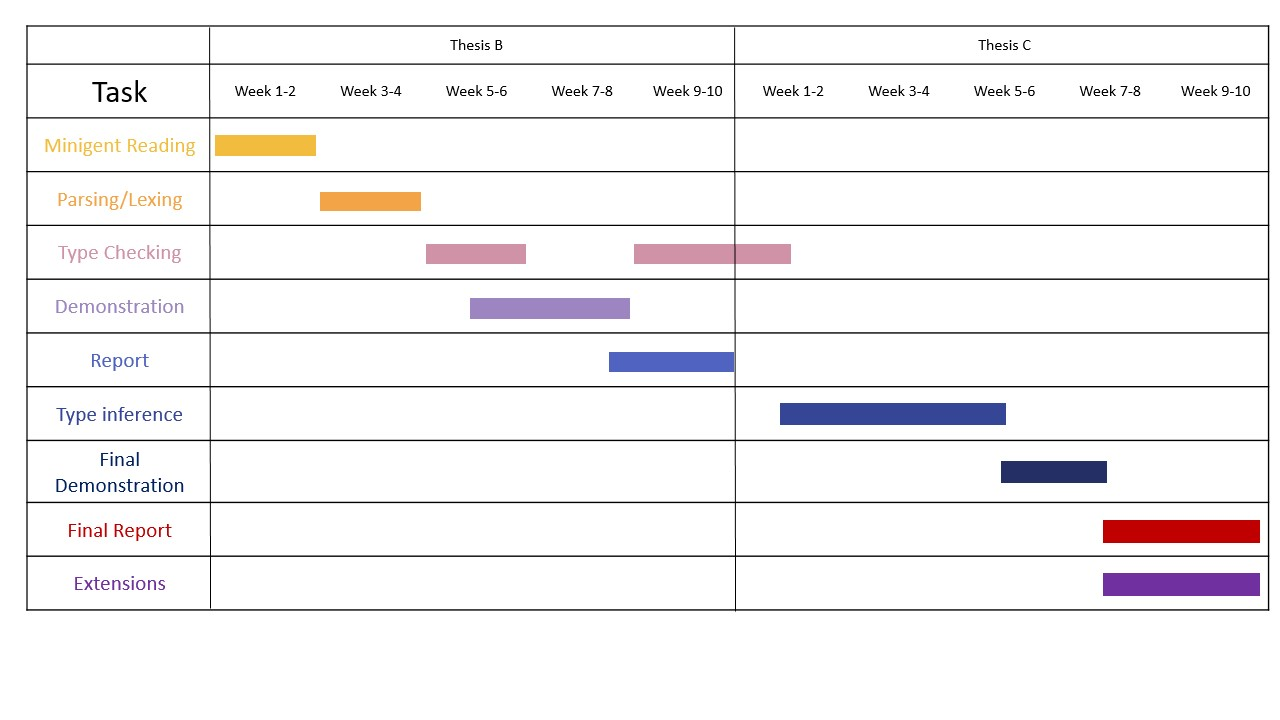
\includegraphics[width=\linewidth]{content/previous_plan.jpg}
    \caption{The previous plan timeline, outlined in thesis A.}
    \label{fig:thesisATimeline}
\end{figure}

\section{Parser and Lexer}

The Minigent lexer and parser now accepts a new recursive parameter extension to boxed records,
as seen in \autoref{fig:recursiveParameter}.

\begin{figure}
    \centering
    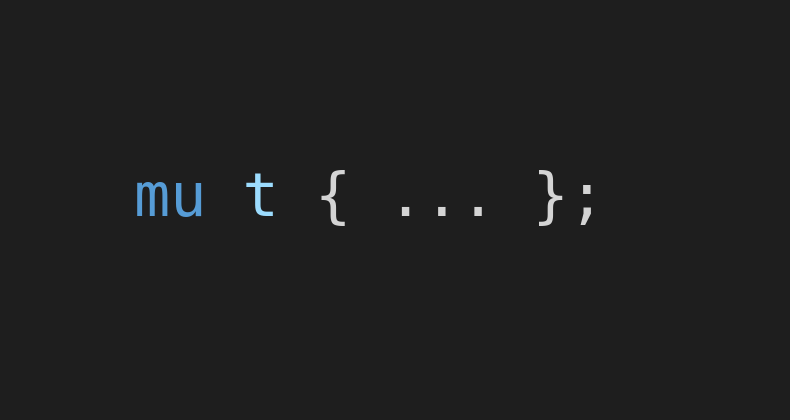
\includegraphics[width=0.5\linewidth]{content/recursive_parameter.png}
    \caption{The new recursive parameter grammar for boxed records}
    \label{fig:recursiveParameter}
\end{figure}

This new syntax is backwards compatible with the previous record syntax, so records without this new
syntax in old code will not have to be changed in order for the change to be implemented.

\todo{Should I talk about the code I wrote here?}

\section{Reorganiser}

In the reorganiser, a strict positivity check has been added to prevent the construction of infinitely
recursive objects. This check recursively evaluates all of the functions in a Minigent program, and
checks that their types do not contain a non-strictly positve type. This check also accounts for the
shadowing of recursive parameter variables, in the event a nested boxed record declaration's recursive
parameter shadows the parent record's parameter. These new recursive parameters are now distinguished from
regular type variables, and the reorganiser no longer counts them as type variables.

\todo{Functions calling themselves}
\todo{Unused recursive parameter variables}

\section{Type Checker}

\todo{Talk about the stuff}

\section{Testing}

\todo{talk about the tests}

\section{Work efficiency}

\todo{talk about syntax highlighting, but also potentially remove}